%-----------------------------------------------------------------------------%
\chapter{\babSatu}
%-----------------------------------------------------------------------------%

Bab ini menjelaskan latar belakang permasalahan, perumusan masalah, tujuan penelitian ini dilakukan, ruang lingkup penelitian serta sistematika penulisan.

%-----------------------------------------------------------------------------%
\section{Latar Belakang}
%-----------------------------------------------------------------------------%

Penggunaan \textit{web} sebagai sarana untuk berbagi informasi pada saat ini sangat tinggi. Namun, tidak banyak orang yang mampu mengembangkan web serta tidak adanya anggaran untuk pembuatan \textit{web} menjadi masalah tersendiri terutama bagi organisasi non-profit. Selain itu, banyaknya informasi yang tersebar di \textit{web} saat ini hanya sebatas informasi saja yang tidak dapat diolah. Hal ini karena informasi-informasi tersebut tidak memiliki hubungan yang terstruktur dan hanya didesain untuk manusia saja sehingga program komputer tidak dapat mengolah informasi tersebut \citep{berners.semantic}.

Selain permasalahan informasi yang tidak dapat diolah oleh komputer, permasalahan lainnya adalah \textit{web} yang ada saat ini kebanyakan memiliki fitur yang sama. Namun, dalam pembuatannya setiap \textit{web} hanya didesain khusus untuk pembuatan satu \textit{web} saja. Tentu saja hal ini dapat dibantu dengan menerapkan paradigma \textit{software product line} dimana \textit{software product line} dapat menghemat biaya produksi, mempercepat waktu produksi ke pasar serta lebih menjadi kualitas dari produk yang dihasilkan \citep{book.sple}.

Pada tahun 2001, \cite{berners.semantic} menemukan sebuah teknologi yang dinamakan \textit{web} semantik, dimana \textit{web} semantik akan membuat sebuah struktur untuk informasi yang terdapat pada \textit{web} sehingga informasi-informasi tersebut dapat diolah oleh program komputer \citep{berners.semantic}. Menurut Rob McCool, Format yang kompleks dan pengguna harus mengorbankan kemudahan ekspresivitas serta membayar biaya yang besar untuk translasi dan perawatan menjadi alasan kenapa \textit{web} semantic tidak akan pernah diadopsi publik secara luas \citep{pragmatic.web}.

Untuk mempermudah proses pembuatan \textit{web} semantik, maka diciptakan \textit{web} pragmatis dimana tujuannya adalah meningkatkan kolaborasi manusia untuk lebih efektif dengan teknologi yang tepat seperti sistem untuk negosiasi ontologi, interaksi bisnis yang terdapat pada ontologi, dan untuk membangun ontologi pragmatis pada praktik masyarakat \citep{pragmatic.web}. Sehingga \textit{web} pragmatis dapat melengkapi \textit{web} semantik untuk berkolaborasi dan meningkatkan kualitas pada level masyarakat.Salah satu perkembangan \textit{web} semantik pragmatis adalah Zotonic, yaitu sebuah framework sekaligus Content Management System (CMS) yang dibangun di atas bahasa pemrograman erlang dimana Zotonic telah mengadopsi konsep \textit{web} semantik. Kehadiran Zotonic sendiri diharapkan dapat meningkatkan pemanfaatan \textit{web} semantik dalam proses pembuatan \textit{web}. sehingga infomasi yang berada pada \textit{web} yang dibuat dapat langsung diolah oleh komputer. Tetapi, pengembang perlu mendefinisikan semantik yang akan mereka buat terlebih dahulu sebelum mereka mengembangkannya dalam Zotonic untuk menciptakan sebuah konsistensi. Namun hal ini tentu saja menghambat proses pengembangan karena pengembang membutuhkan waktu yang lebih lama untuk proses translasi dari semantik ke Zotonic.

Untuk membantu para pengembang dalam mentranslasikan semantik ke dalam Zotonic, pada tahun 2016 terdapat sebuah penelitian terkait pembentukan otomatis aplikasi \textit{web} dengan masukan berupa ontologi, yaitu penelitian terkait pemetaan ontologi yang dihasilkan semantik ke dalam struktur Zotonic \citep{bravyto}. Namun, pada penelitian tersebut pembentukan \textit{business logic} dari \textit{web} yang dibentuk masih secara manual. Hal ini dikarenakan pada ontologi tidak terdapat \textit{business logic} sehingga tidak dapat secara otomatis. \textit{Business logic} tersebut dapat diperoleh dari ABS \textit{microservices} seperti pada \pic~\ref{fig:roadmapbab1}.

\begin{figure}
	\centering
	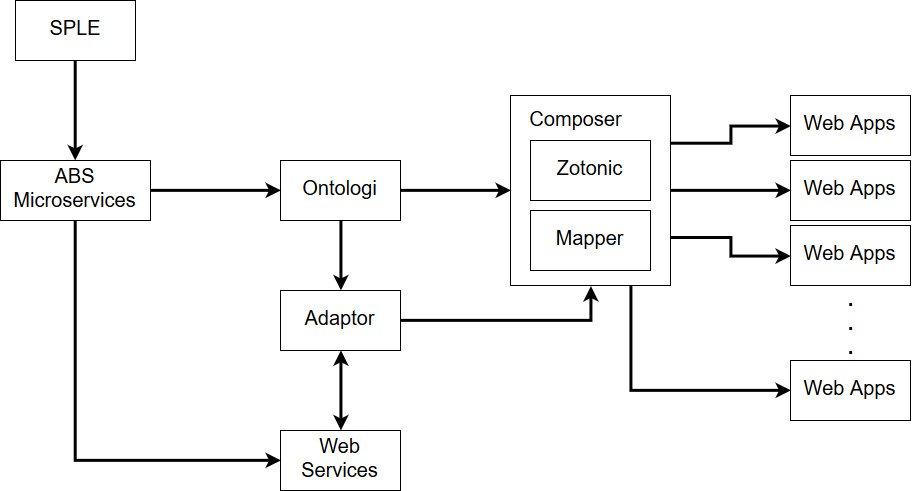
\includegraphics[width=1\textwidth]
	{pics/roadmapbab1.jpg}
	\caption{\textit{Roadmap} pembentukan \textit{web} berbasis semantik}
	\label{fig:roadmapbab1}
\end{figure}
\vspace{-0.3cm}

Dengan memanfaatkan ABS \textit{microservices} yang dihasilkan dari SPLE, maka tidak hanya membuat sebuah \textit{web} berbasis semantik saja tetapi Zotonic yang dihasilkan nantinya dapat membuat beberapa \textit{web} berbasis semantik yang memiliki struktur yang sama yang berasal dari ontologi dan \textit{business logic} yang dapat disesuaikan dengan kebutuhannya. Oleh karena itu, penting untuk dilakukan penelitian mengenai bagaimana cara menghubungkan ontologi tersebut dengan \textit{web services} pada Zotonic agar lebih memudahkan dan lebih efisien dalam pembuatan \textit{web}.
%-----------------------------------------------------------------------------%
\section{Perumusan Masalah}
%-----------------------------------------------------------------------------%
Berdasarkan latar belakang tersebut, penelitian ini akan mencoba untuk menjawab beberapa pertanyaan penelitian, yaitu
\begin{enumerate}
\item Bagaimana proses integrasi ontologi kepada \textit{web service}?
\item Apakah dapat dikembangkan sebuah program \textit{adaptor} yang akan melakukan integrasi ontologi dan \textit{web service} secara otomatis?
\end{enumerate}
%-----------------------------------------------------------------------------%
\section{Tujuan Penelitian}
%-----------------------------------------------------------------------------%
Tujuan dari penelitian ini adalah untuk mengembangkan sebuah program yang dapat menghubungkan antara \textit{web services} dan Zotonic sehingga proses pembuatan \textit{site} pada Zotonic dapat memiliki tingkat adaptasi yang baik terhadap perubahan yang terjadi. Harapannya melalui program yang dibuat, pengembang dapat tetap fokus untuk \textit{maintain} data dan mengembangkan aplikasi, karena data sudah terjadi melalui ontologi.

%-----------------------------------------------------------------------------%
\section{Ruang Lingkup Penelitian}
%-----------------------------------------------------------------------------%

Ruang lingkup penelitian ini antara lain:
\begin{enumerate}
\item Analisis pemetaan \textit{adaptor} untuk menghubungkan antara ontologi dan \textit{web service}.
\item Perancangan sistem yang dapat menghubungkan antara ontologi dan \textit{web service} melalui Zotonic.
\item \textit{Refactoring} pembuatan \textit{business logic} yang sudah ada dengan memanfaatkan sistem yang dibuat.
\end{enumerate}

%-----------------------------------------------------------------------------%
\section{Sistematika Penulisan}
%-----------------------------------------------------------------------------%
Sistematika penulisan laporan adalah sebagai berikut:
\begin{itemize}
	\item Bab 1 \babSatu
	
	Bab 1 berisi tentang informasi terkait penelitian yang dilakukan oleh penulis, dimana bab ini terdiri atas 5 subbab, yaitu latar belakang, perumusan masalah yang akan diteliti oleh penulis, tujuan penelitian, ruang lingkup penelitian serta sistematika penulisan.\\
	\item Bab 2 \babDua
	
	Bab 2 berisi mengenai penjelasan terkait ontologi, \textit{web} \textit{framewok} berbasis semantic: Zotonic, dan \textit{software product line}.\\
	\item Bab 3 \babTiga 
	
	Bab 3 berisi penjelasan mengenai rancangan dari sistem yang akan diimplementasikan, dimana bab ini terdiri atas 3 subbab, yaitu rancangan integrasi ontologi dan \textit{web service}, rancangan \textit{web service} serta rancangan \textit{adaptor}.\\
	
	\item Bab 4 \babEmpat
	
	Bab 4 berisi penjelasan mengenai impelementasi yang dilakukan oleh penulis untuk membuat \textit{adaptor}. \\
	
	\item Bab 5 \babLima	
	
	Bab 5 berisi perubahan yang terjadi setelah eksperimen dan hasil uji coba eksperimen yang telah dilakukan oleh penulis. \\
	
	\item Bab 6 \babEnam
	
	Bab 6 berisi kesimpulan yang didapat dari penelitian serta saran yang diajukan untuk penelitian berikutnya.
\end{itemize}